\documentclass[conference]{IEEEtran}
\IEEEoverridecommandlockouts
\pagestyle{plain}   % NDSS: page numbers on

% --- IEEE / Basic packages ---
\usepackage{cite}
\usepackage{amsmath, amssymb}
\usepackage{algorithm}
\usepackage[noend]{algpseudocode}
\usepackage{graphicx}
\usepackage{textcomp}
\usepackage{xcolor}    % IEEEtran (unlike ieeecolor) does not auto-load a color pkg
\usepackage{colortbl}  % for \rowcolor in tables
\definecolor{lightgray}{gray}{0.85}  % replacement for xcolor's gray!15
\let\proof\relax
\let\endproof\relax
\usepackage{amsthm}
\newtheorem{lemma}{Lemma}
\newtheorem{proposition}{Proposition}
\usepackage{ragged2e}
\usepackage{booktabs}
\usepackage{makecell}
\usepackage{multirow}
\usepackage{float}
\newtheorem{theorem}{Theorem}
\newtheorem{corollary}{Corollary}
\newtheorem{remark}{Remark}
\newtheorem{definition}{Definition}
\newcommand{\tblstyle}{\small\setlength{\tabcolsep}{4pt}}

% --- Float spacing (IEEEtran journal defaults) ---

\def\BibTeX{{\rm B\kern-.05em{\sc i\kern-.025em b}\kern-.08em
    T\kern-.1667em\lower.7ex\hbox{E}\kern-.125emX}}

\begin{document}

\title{PETSE: A Probabilistic Execution-Time Safety Envelope with Continuous Runtime Re-Verification for Mobile Robots}

% Double-blind submission: authors anonymized for review
\author{\IEEEauthorblockN{Anonymous Author(s)}
\IEEEauthorblockA{Paper \#XXX --- Submitted to NDSS 2026}}

% --- NDSS 2026 publication ID block (per bare_conf_NDSS2026 template) ---
\makeatletter\def\@IEEEpubidpullup{6.5\baselineskip}\makeatother
\IEEEpubid{\parbox{\columnwidth}{
    Network and Distributed System Security (NDSS) Symposium 2026\\
    23 - 27 February 2026, San Diego, CA, USA\\
    ISBN 979-8-9919276-8-0\\
    https://dx.doi.org/10.14722/ndss.2026.[23$|$24]xxxx\\
    www.ndss-symposium.org
}\hspace{\columnsep}\makebox[\columnwidth]{}}

\maketitle
\IEEEpubidadjcol

\begin{abstract}
A navigation task that is safe when an operator---or a large language model (LLM) front-end---approves it can still become unsafe during execution: localization can be spoofed \emph{after} the safety check (a time-of-check to time-of-use gap), tracking error and latency can drift the robot off its approved path, and braking overshoot can carry it past a boundary. Prompt- and planning-stage defenses check a task once, at approval time, and cannot revoke that approval once motion begins. This article presents PETSE (Probabilistic Execution-Time Safety Envelope), an execution-layer module that \emph{continuously re-verifies} an already-approved task against spatial constraints at every control cycle, revoking approval and stopping the robot the moment its true state violates the constraint. A probabilistic safety envelope---the sum of four physically grounded bounds (pose-covariance radius, cross-track error, latency-induced displacement, and kinematic braking distance)---sets the re-verification threshold, but the load-bearing mechanism is the continuous monitor itself. In a paired factorial experiment that holds this margin \emph{fixed}, disabling the runtime monitor turns 100\,\% of post-approval attacks into zone violations ($0/10 \rightarrow 10/10$ violated), whereas the full monitor closes this attack surface (100\,\%~$\rightarrow$~0\,\%); the outcome is identical under two structurally different Nav2 local planners (DWB and RPP), confirming an execution-layer property rather than a controller artifact. Across a 20-seed Gazebo campaign over four cyber-physical attack scenarios, PETSE attains 100\,\% detection recall with a 0.0\,\% zone-violation rate, never nuisance-trips 243 benign trajectories, and halts every intervention with positive clearance at 147\,$\mu$s per-cycle overhead. Hardware tests on a Jetson-class Ackermann-steering car with dead-reckoning odometry show that the measured safety gap is consistent with the formula-predicted margin.
\end{abstract}

\begin{IEEEkeywords}
Runtime assurance, runtime safety monitor, time-of-check to time-of-use, cyber-physical security, dynamic safety margin, industrial mobile robots, LLM-enabled robotics
\end{IEEEkeywords}

%=====================================================================
\section{Introduction}
%=====================================================================

\IEEEPARstart{I}{ndustrial} mobile robots---particularly those in semiconductor fabs---operate alongside restricted zones whose unauthorized entry risks both physical harm and confidentiality breaches. Recent work has shown that large language models (LLMs) can serve as natural-language front-ends that translate operator commands into navigation goals~\cite{ahn2023do,liang2023code,singh2023progprompt,huang2023inner,huang2022language}, greatly improving usability but simultaneously opening a new attack surface in the control pipeline.

Because an LLM accepts arbitrary text, an adversary can craft prompts that produce navigation goals pointing straight into a forbidden zone~\cite{perez2022ignore,greshake2023not,robey2025jailbreaking}. In a conventional stack, injecting such goals requires access to internal communication channels; an LLM-based interface lowers this barrier dramatically~\cite{yaacoub2022robotics}.

Execution-time disturbances---localization drift, cross-track error, and communication delay---compound the risk. Current defenses act at the prompt or planning stage: post-validation~\cite{yang2024plug}, LTL plan constraints~\cite{wu2025selp}, and shielding~\cite{alshiekh2018safe}. Once a plan has been approved, however, none of these mechanisms can intervene if the robot deviates from the planned path during execution.

PETSE closes this gap at the execution layer. Rather than approving a task once and trusting it thereafter, PETSE treats an approval as \emph{revocable}: it re-verifies the already-approved task against the spatial constraint at every control cycle, using the robot's live uncertainty state, and revokes the approval---stopping the robot through a trusted stop channel---the moment its true position would violate the constraint. A probabilistic safety envelope sets the threshold for this check, but the continuous re-verification is what catches failures that arise \emph{after} approval, which no prompt- or planning-stage check can address. The main contributions of this article are summarized as follows.
\begin{enumerate}
\item \textbf{Revocable approval via continuous runtime re-verification.}
We cast execution-layer safety as the continuous re-verification of an already-approved task, so an approval can be revoked mid-execution when the robot drifts off its safe path---through localization spoofing after the check (a time-of-check to time-of-use gap), tracking error, latency, or braking overshoot. A paired factorial experiment that holds the margin fixed shows this monitor, not the margin width, is what closes the post-approval attack surface (100\,\%~$\rightarrow$~0\,\% violations).

\item \textbf{Uncertainty-aware safety envelope.}
Four physically grounded bounds---localization covariance, cross-track error, latency drift, and braking distance---are summed into an additive margin that envelopes every reachable true position and sets the re-verification threshold from an operator-specified violation tolerance~$\varepsilon$.

\item \textbf{Controller-agnostic execution-layer module (three gates).}
A drop-in ROS~2 node applies a goal gate, a path gate, and a per-cycle runtime monitor without altering any navigation component; the runtime monitor acts on the command channel and its guarantee is validated identically under two different local planners (DWB and RPP).

\item \textbf{Attack model with demonstrated realizability.}
We organize six attack scenarios into a capability ladder (Table~\ref{tab:ladder})---from command-tier goal injection that needs no robot access, through unauthenticated \texttt{cmd\_vel} injection and physical map-consistent LiDAR spoofing, to coordinated dual-channel compromise---and empirically confirm the network rung on a default ROS~2 stack, where an unprivileged process with no security material injects drive commands over unauthenticated DDS. This delimits precisely which attacks an execution-layer monitor can and cannot address.

\item \textbf{Causal and systematic evaluation.}
Beyond a multi-seed campaign over six cyber-physical attack scenarios in simulation and on hardware---including a localization-spoofing hijack that defeats every planning-layer baseline ($5/5$ zone entries) while PETSE holds ($0/5$)---we isolate the runtime monitor with a paired ablation, characterize the attack-surface boundary with a magnitude sweep, and report the monitor's operating point (zero nuisance trips on benign runs; positive stopping clearance on every intervention).
\end{enumerate}

The rest of this article is organized as follows. Section~II reviews related work. Section~III defines the threat model and attack scenarios. Section~IV details the proposed method. Section~V presents experimental results including simulation and real-robot validation. Section~VI discusses limitations, and Section~VII concludes this article.

%=====================================================================
\section{Background and Related Work}
%=====================================================================

\begin{figure*}[t]
    \centering
    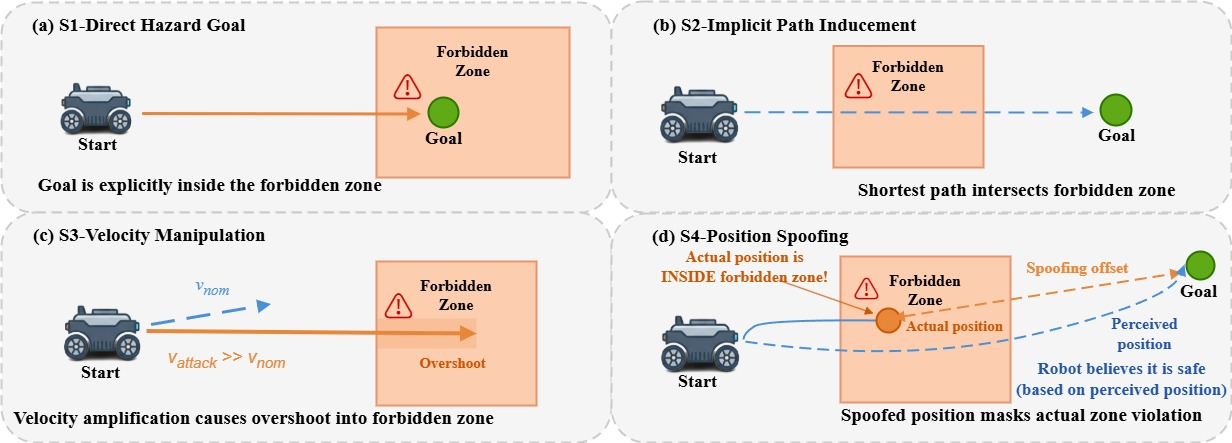
\includegraphics[width=0.88\textwidth]{attack_scenarios_s1s4_v2.jpg}
    \vspace{-2ex}
    \caption{Overview of four cyber-physical attack scenarios (S1--S4) targeting different layers of the LLM-enabled robot control pipeline.}
    \label{fig:attack_scenarios}
    \vspace{-2ex}
\end{figure*}

\subsection{LLM-based Robot Planning and Safety}
Recent studies show that LLMs can ground affordance reasoning, generate multimodal plans, and synthesize task-level policies for robots~\cite{ahn2023do,liang2023code,singh2023progprompt,huang2023inner,huang2022language,driess2023palm,brohan2023rt}. Yet none of these pipelines verifies that the resulting motion remains physically safe once execution begins---a critical omission when localization noise, network delay, or adversarial perturbation can push the robot off its planned path. In semiconductor fabs or pharmaceutical facilities, a single unauthorized zone entry may disrupt production or leak proprietary layout information.

\subsection{Safety Mechanisms for LLM-enabled Robots}
SafetyChip~\cite{yang2024plug} appends a post-hoc verification step to LLM-generated actions; SELP~\cite{wu2025selp} constrains plans with linear temporal logic (LTL); shielding~\cite{alshiekh2018safe} filters unsafe discrete actions before they reach the executor. Robey et al.~\cite{robey2025jailbreaking} demonstrated that adversarial prompts routinely bypass these prompt-level filters.

All four methods sit at or above the planning layer: once a plan is approved, they have no mechanism to intervene when spoofed localization, injected latency, or accumulated tracking error drives the robot off course. PETSE fills this gap by operating one layer below---at execution time---and is designed to complement, not replace, planning-stage defenses.

\subsection{Control-theoretic and Spatial Safety Approaches}
Control Barrier Functions (CBFs)~\cite{ames2017control,ames2019control} solve a quadratic program at each control step to keep the state inside a certified safe set, but they rely on accurate dynamics models and trustworthy state feedback. Speed and Separation Monitoring (SSM)~\cite{iso2016robots,marvel2017implementing} adjusts human--robot distance per ISO/TS~15066~\cite{rosenstrauch2017safe}, while geofencing~\cite{stevens2021geofence,vagal2021new} enforces hard spatial boundaries and has been studied mainly for GPS-equipped UAS~\cite{villani2018survey}.

Each approach has a specific blind spot. CBF cannot detect a spoofed state and does not check whether the \emph{planned path} crosses a forbidden zone; our experiments in Section~\ref{sec:experiments} confirm that control-channel attacks invalidate its guarantee. SSM ignores localization uncertainty and network delay, limiting its use with static indoor forbidden zones. Conventional geofences assume centimeter-accurate positioning, an assumption that breaks down under AMCL in cluttered indoor environments.

PETSE sidesteps these issues by sitting \emph{outside} the control loop as a purely geometric monitor. It inflates each forbidden polygon by a dynamic margin built from AMCL covariance~\cite{fox1999monte,fox2003adapting}, cross-track error, and worst-case latency drift, and then (i)~blocks or projects goals that fall inside the inflated zone, (ii)~rejects paths that intersect it, and (iii)~continuously verifies the distance constraint at every control cycle. Because PETSE never modifies the control input, it cannot destabilize the controller; the cost of this design is purely reactive intervention, which is acceptable for a last-resort safety layer.

\begin{table}[t]
\centering
\caption{Comparison of safety approaches for LLM-enabled robots.}
\label{tab:related}
\footnotesize
\begin{tabular}{@{}l c c c c@{}}
\toprule
Method & Layer & \makecell{Uncertainty\\Aware} & \makecell{Attack\\Robust} & \makecell{Dynamic\\Margin} \\
\midrule
SafetyChip~\cite{yang2024plug} & Planning & \texttimes & \texttimes & \texttimes \\
SELP~\cite{wu2025selp} & Planning & \texttimes & \texttimes & \texttimes \\
Shielding~\cite{alshiekh2018safe} & Planning & \texttimes & \texttimes & \texttimes \\
CBF~\cite{ames2017control,ames2019control} & Control & \texttimes$^{*}$ & \texttimes & \checkmark \\
SSM~\cite{iso2016robots,marvel2017implementing} & Control & \texttimes & \texttimes & \texttimes \\
Static Geofence~\cite{stevens2021geofence,vagal2021new} & Execution & \texttimes & \texttimes & \texttimes \\
\rowcolor{lightgray} \textbf{Ours} & \textbf{Execution} & \checkmark & \checkmark & \checkmark \\
\bottomrule
\multicolumn{5}{@{}l}{\footnotesize $^{*}$CBF handles model uncertainty but not localization uncertainty.}
\end{tabular}
\end{table}

Table~\ref{tab:related} positions PETSE against these baselines. No prior method that we are aware of derives a dynamic execution-layer margin from the joint contribution of localization covariance, tracking error, and communication latency.

%=====================================================================
\section{Threat Model and Attack Scenarios}
%=====================================================================

\subsection{System and Threat Model}\label{sec:threat_model}
We consider a wheeled mobile robot navigating an indoor industrial
facility whose forbidden zones $F$ are specified as closed polygons.
The true pose $p_t$ is estimated as $\hat{p}_t$ by AMCL from an
\emph{exteroceptive} channel (LiDAR matched against a known map),
subject to non-negligible localization error and end-to-end
communication delay. The software stack is layered: an upper
command-generation tier (including the LLM) emits navigation goals that
a lower execution tier carries out. In parallel, a \emph{proprioceptive}
channel---wheel odometry $o_t$ computed on-board from motor encoders
(\texttt{/odom})---provides an independent estimate of incremental
motion.

\textbf{Adversary.} A cyber-physical adversary~\cite{yaacoub2022robotics}
may (i)~inject or contaminate navigation goals at the command tier
(prompt injection, context poisoning); (ii)~tamper with control
parameters or inflate the communication latency of the execution tier;
and (iii)~corrupt the \emph{exteroceptive} perception channel, e.g., by
physically spoofing the LiDAR return so that $\hat{p}_t$ appears safe
while $p_t$ drifts toward $F$~\cite{cao2019adversarial,sun2020towards}.
The adversary can neither actuate the motors or rewrite low-level
firmware, nor---the load-bearing assumption---consistently corrupt the
on-board proprioceptive odometry $o_t$ and the enforcement node's own
compute.

\textbf{Realizability of the cyber capabilities.} Capabilities (i)--(ii)
reduce to reaching the robot's ROS~2 graph and publishing to its command
or control topics, which is realistic \emph{without} firmware or root
access. ROS~2's default DDS middleware ships with authentication and
encryption disabled unless SROS2/DDS-Security is explicitly
configured~\cite{mayoralvilches2022sros2,diluoffo2018ros2}, and DDS
endpoints have been found unauthenticated and even exposed on the public
Internet~\cite{maggi2022dds}; remote compromise of an industrial robot
controller over the network has been demonstrated
end-to-end~\cite{quarta2017experimental}, unauthorized topic publication
and man-in-the-middle attacks against ROS have been
shown~\cite{dieber2017security}, and exposed robots are automatically
discoverable by footprinting tools~\cite{mayoralvilches2018aztarna}. We
confirmed this on our own stack: on a default ROS~2 (Jazzy, Fast-DDS,
SROS2 off), an unprivileged process with no security material discovers
the \texttt{/cmd\_vel} topic through unauthenticated DDS discovery and
injects $1.5$\,m/s drive commands that the base controller accepts.
An attacker who merely reaches the robot's network---e.g., over Wi-Fi or
from a co-located device---therefore obtains the command/control-tier
capabilities of S1--S4 without touching low-level firmware or the
proprioceptive channel that anchors PETSE.

\textbf{Trust anchor and scope (A1).} PETSE re-verifies safety by
cross-checking the exteroceptive estimate $\hat{p}_t$ against the
independent proprioceptive channel $o_t$; its guarantee therefore holds
\emph{as long as at least one of the two channels remains honest}, which
Assumption~A1 formalizes: $o_t$ and the monitor compute are
uncompromised. A1 is well matched to the threat that motivates this
work: a \emph{remote} sensor-spoofing attacker reaches the LiDAR by line
of sight but cannot touch odometry, which is computed on-board from
encoders it does not control. An attacker who \emph{also} corrupts $o_t$
so that $\hat{p}_t$ and $o_t$ agree on a false pose to within the safety
margin must first compromise the on-board compute; such a privileged
adversary is \emph{out of scope} and is properly addressed by an
independent, physically separated safety channel---a safety-rated PLC or
a pose-independent boundary sensor (e.g., a light curtain)---following
standard functional-safety practice. Crucially, merely \emph{disabling}
the monitor is not a bypass: the enforcement guard is the sole publisher
on the actuation channel that reaches the motors, so crashing, killing, or
detaching it removes all motor commands and the platform coasts to a
fail-stop rather than moving freely. A heartbeat/watchdog on the safety
controller---which disarms the drive on loss of a valid monitor
attestation---makes this fail-\emph{closed} behavior explicit. Thus
``switching PETSE off'' is self-defeating: turning the monitor off closes
the only path into $F$, whereas reaching $F$ requires keeping the monitor
\emph{running yet deceived}---precisely the consistent dual-channel
spoofing that A1 delimits. Notably, the security boundary is
set not by the mere \emph{presence} of privilege but by whether PETSE's
trust anchor (an honest $o_t$) survives; we characterize this boundary
empirically in Section~\ref{sec:coord}, showing that PETSE is evaded only
once the residual cross-channel disagreement is driven below the margin,
i.e., only under consistent dual-channel spoofing.

The four scenarios below span the in-scope capability range: S1 and S2
require only \emph{untrusted input} to the command tier and no robot
access; S3 requires \emph{write access} to control parameters or the
communication channel; and S4 corrupts a \emph{single exteroceptive
channel} and, in its canonical LiDAR-spoofing form, is realizable
remotely without on-board access. In every in-scope case the
proprioceptive odometry remains an honest reference, which is precisely
what lets an execution-layer cross-check revoke an already-approved task.

\subsection{Attack Scenarios}
Six scenarios target distinct control layers (Fig.~\ref{fig:attack_scenarios}) to force the robot into forbidden zone~$F$. For each we state not only the mechanism but the \emph{capability it requires} and \emph{how that capability is realistically obtained}; Table~\ref{tab:ladder} summarizes the resulting ladder. S1--S4 are the core factorial campaign; S5--S6 stress execution-time defenses specifically.

\textbf{S1 (Direct Hazard Goal).} Coordinates inside $F$ are injected as the navigation goal via prompt injection or command contamination. \emph{Capability:} untrusted input to the command tier only---no robot access. It probes whether the safety layer blocks or reprojects overtly dangerous goals.

\textbf{S2 (Implicit Path Inducement).} Start and goal both lie outside $F$, yet the shortest feasible path cuts through it. \emph{Capability:} same command-tier input as S1; the attack exploits planner geometry, exposing defenses that inspect only the goal coordinate and not the trajectory.

\textbf{S3 (Velocity Manipulation + Communication Delay).} The approved goal is safe, but the attacker amplifies execution velocity and injects 0--100\,ms of extra latency so that cumulative displacement overshoots the planned envelope. \emph{Capability:} write access to control parameters or the communication channel---i.e., a network foothold on the ROS~2 graph (Section~\ref{sec:threat_model}).

\textbf{S4 (Position Spoofing).} The localization estimate $\hat{p}_t$ is offset so it appears safe while the true position $p_t$ drifts toward $F$. Two realizations bracket the capability range. \emph{(a) \texttt{cmd\_vel} injection:} an unprivileged process publishes drive commands over unauthenticated DDS (Section~\ref{sec:threat_model}), requiring only network reach. \emph{(b) Map-consistent LiDAR spoofing:} the attacker injects crafted laser returns~\cite{sun2020towards,cao2019adversarial} that, ray-cast from a chosen spoofed pose against the \emph{known} facility map, form a self-consistent scan; AMCL converges to the spoofed pose. This needs only physical line-of-sight to the sensor---no software intrusion and no access to the proprioceptive odometry that anchors PETSE.

\textbf{S5 (Localization-Spoofing Hijack, TOCTOU).} A composite, security-motivated scenario: a hijacked robot is steered into a confidential keep-out zone (e.g., to film fab interior). The goal is approved on a clean pose; \emph{during} execution, map-consistent LiDAR spoofing (S4b) biases $\hat{p}_t$ so the robot appears to stay clear while $p_t$ enters $F$---a time-of-check-to-time-of-use gap that goal- and path-level approval cannot revoke. \emph{Capability:} S4b (physical line-of-sight), no on-board compromise.

\textbf{S6 (Time-Varying Forbidden Zone).} The keep-out region changes after approval: a zone is \emph{activated mid-navigation}, after the goal was cleared on a then-unobstructed path (dynamic safety areas, shift changes, human co-presence). \emph{Capability:} none beyond a legitimate zone update---it needs no attacker at all, yet defeats any approval-time-only check, isolating the value of continuous re-verification.

\begin{table}[t]
\centering\footnotesize
\caption{Attacker capability ladder. Each scenario's required capability and how it is realistically obtained. Only consistent dual-channel compromise (bottom, per~A1) is out of scope; PETSE defends every rung above it.}
\label{tab:ladder}
\setlength{\tabcolsep}{3pt}
\renewcommand{\arraystretch}{1.15}
\begin{tabular}{@{}p{1.35cm} p{2.35cm} p{2.5cm} c@{}}
\toprule
Attack & Capability required & Realized by & PETSE \\
\midrule
S1--S2 goal inj. & Untrusted input to command tier & Prompt injection; no robot access & \checkmark \\
S3 param/lat. & Write to params / comms & Network foothold on ROS~2 graph & \checkmark \\
S4a \texttt{cmd\_vel} & Publish to actuation topic & Unauth.\ DDS on robot net~\cite{maggi2022dds,dieber2017security} & \checkmark \\
S4b/S5 LiDAR spoof & Corrupt one exteroceptive channel & Laser injection, physical LoS, no SW~\cite{sun2020towards,cao2019adversarial} & \checkmark \\
S6 t-var zone & None (legit.\ zone update) & Post-approval activation & \checkmark \\
\midrule
Coord.\ dual-ch. & On-board compute \emph{and} odom & Root / firmware compromise & $\times$\,(A1) \\
\bottomrule
\end{tabular}
\end{table}

%=====================================================================
\section{Proposed Method}
%=====================================================================

The central contribution of PETSE is a \emph{mechanism}, not a formula: a runtime monitor that re-evaluates an already-approved task against its spatial constraint at \emph{every} control cycle. An attack injected \emph{after} approval---when prompt- and planning-stage checks are no longer in the loop---is caught the moment the robot's estimated state approaches a forbidden zone, because the check is repeated continuously rather than once. The safety margin derived in Section~\ref{sec:margin} is not the contribution in itself; it only sets the distance threshold this monitor enforces, chosen conservatively enough that the check never fires late. Accordingly, we first describe the enforcement architecture (Section~\ref{sec:architecture}) and then the margin that parameterizes it (Section~\ref{sec:margin}); the experiments (Section~\ref{sec:reverify}) confirm that it is the continuous re-verification---not the particular margin value, which is held \emph{fixed} across the key ablation---that closes the post-approval attack surface.

\subsection{System Architecture}\label{sec:architecture}
Fig.~\ref{fig:system_arch} illustrates the four-layer pipeline and the position of the PETSE enforcement layer within the overall control architecture.

\subsubsection{Pipeline Layers}
\textbf{Layer~1 --- Natural-language command.}
An operator issues a task instruction in free-form text (e.g., ``Deliver the tray to Zone~C''). The LLM parses the instruction, resolves spatial references, and outputs a 2D navigation goal $g=(x,y)$.

\textbf{Layer~2 --- Planning.}
The navigation planner (Nav2~\cite{macenski2020marathon}) receives $g$ and computes a collision-free path $\pi = \langle p_1,\dots,p_n \rangle$ using the global costmap and AMCL pose estimate.

\textbf{Layer~3 --- Execution.}
The local controller (e.g., DWB or Regulated Pure-Pursuit) tracks $\pi$ by publishing velocity commands to the mobile base at the control frequency (typically 20--50\,Hz).

\textbf{Layer~4 --- PETSE enforcement.}
The PETSE node intercepts the data flow between Layers~2--3 and the localization subsystem. It neither trusts the semantic content of LLM outputs nor modifies any upstream module. At each control cycle it reads the current pose estimate and covariance, recomputes the dynamic safety margin, and checks whether the robot could reach a forbidden zone within the decision-to-stop horizon. If the check fails, PETSE blocks the goal, projects it to the nearest safe point, or commands an immediate stop.

\subsubsection{ROS\,2 Integration}
PETSE is implemented as a single ROS\,2 lifecycle node that can be inserted into an existing Nav2 deployment without modifying any upstream package. Table~\ref{tab:ros} lists the subscribed and published interfaces.

On the input side, the node subscribes to (i)~the AMCL pose with covariance (\texttt{/amcl\_pose}), from which $\hat{p}_t$ and $\Sigma_t$ are extracted, (ii)~the odometry topic (\texttt{/odom}) for the current velocity $v_t$, (iii)~the navigation goal (\texttt{/goal\_pose}) issued by the LLM or operator, and (iv)~the planned global path (\texttt{/plan}) produced by the Nav2 planner.

On the output side, PETSE publishes a filtered goal (\texttt{/petse/safe\_goal}) that is either the original goal (ALLOW), a boundary-projected replacement (PROJECT), or an empty message (REJECT). It also publishes a zero-velocity override (\texttt{/cmd\_vel}) when the runtime monitor triggers an emergency stop, and a diagnostic topic (\texttt{/petse/status}) that reports the current margin $M(t)$, the minimum distance to each forbidden zone, and the enforcement decision at every cycle.

Forbidden-zone polygons are loaded from a YAML parameter file at node startup and can be updated at runtime via a ROS\,2 parameter service without restarting the node. All margin parameters ($v_{\max}$, $\tau$, $a_{\max}$, $\varepsilon$, $e_0$, $c_1$, $\bar\lambda$) are likewise exposed as dynamic parameters, enabling operators to adjust the safety--availability trade-off during deployment.

\begin{table}[t]
\centering
\footnotesize
\caption{ROS\,2 interfaces of the PETSE node.}
\label{tab:ros}
\setlength{\tabcolsep}{3pt}
\begin{tabular}{@{}l l l l@{}}
\toprule
Dir. & Topic & Msg.\ Type & Data \\
\midrule
Sub & \texttt{/amcl\_pose} & \texttt{PoseWithCov.*} & $\hat{p}_t$, $\Sigma_t$ \\
Sub & \texttt{/odom} & \texttt{Odometry} & $v_t$ \\
Sub & \texttt{/goal\_pose} & \texttt{PoseStamped} & $g=(x,y)$ \\
Sub & \texttt{/plan} & \texttt{Path} & $\pi$ \\
\midrule
Pub & \texttt{/petse/safe\_goal} & \texttt{PoseStamped} & Filtered goal \\
Pub & \texttt{/cmd\_vel} & \texttt{Twist} & Zero-velocity override \\
Pub & \texttt{/petse/status} & \texttt{DiagnosticArray} & $M(t)$, decision \\
\bottomrule
\multicolumn{4}{@{}l}{\footnotesize *\texttt{PoseWithCovarianceStamped} (geometry\_msgs).}
\end{tabular}
\end{table}

\begin{figure*}[t]
    \centering
    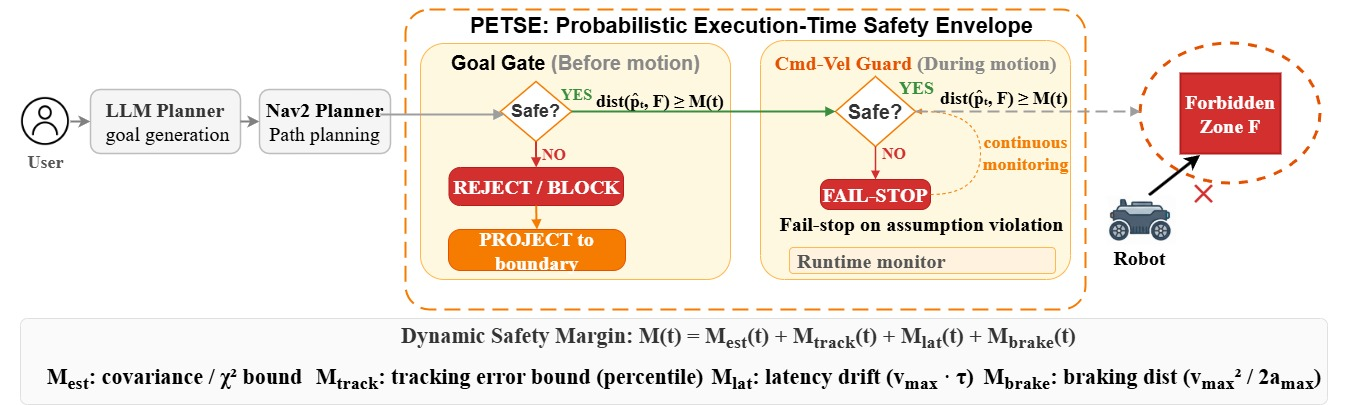
\includegraphics[width=\textwidth]{overview.jpg}
    \vspace{-2ex}
    \caption{System architecture of the proposed PETSE.}
    \label{fig:system_arch}
    \vspace{-2ex}
\end{figure*}

\subsection{Dynamic Safety Margin Formulation}\label{sec:margin}

This section derives the distance threshold $M(t)$ that the runtime monitor of Section~\ref{sec:architecture} enforces. The margin is a means to an end: it must be large enough that a stop issued when $\mathrm{dist}(\hat p_t,\mathcal F)=M(t)$ still halts the robot outside the zone despite localization error, tracking error, latency, and braking. We therefore bound each of these four displacement sources from measurable system parameters and sum them.

\subsubsection{Safety Margin Definition}
Let $p_t \in \mathbb{R}^2$ denote the robot's true position and $\hat{p}_t$ the AMCL estimate at decision time~$t$. The dynamic safety margin is defined as
\begin{equation}
M(t) = M_{\mathrm{est}}(t) + M_{\mathrm{track}}(t) + M_{\mathrm{lat}}(t) + M_{\mathrm{brake}}(t).
\label{eq:margin}
\end{equation}
Each summand upper-bounds one source of Euclidean deviation between $\hat{p}_t$ and the true position over the decision-to-stop interval $[t,\, t{+}\tau{+}t_b]$, with $\tau$ the worst-case latency and $t_b$ the braking time.

\subsubsection{Margin Components}\label{sec:components}

\paragraph{Estimation uncertainty ($M_{\mathrm{est}}$)}
This term caps the gap between the true pose and the AMCL~\cite{fox1999monte,fox2003adapting} estimate. With 2D position covariance $\Sigma_t \in \mathbb{R}^{2\times2}$, the error $e_t := p_t - \hat{p}_t$ obeys $e_t^\top \Sigma_t^{-1} e_t \ge \|e_t\|^2 / \lambda_{\max}(\Sigma_t)$ via the spectral bound. Choosing a risk tolerance $\varepsilon$ gives
\begin{equation}
M_{\mathrm{est}}(t) = \sqrt{\chi^2_{2,\,1-\varepsilon}\,\lambda_{\max}(\Sigma_t)}.
\end{equation}
Geometrically, this replaces the covariance ellipse with a circumscribing circle---a conservative but isotropic bound. Under a Gaussian localization model~\cite{thrun2005probabilistic}, the squared Mahalanobis distance~\cite{mahalanobis1936generalized} is $\chi^2_2$-distributed, so the true position falls within radius $M_{\mathrm{est}}$ of the estimate with probability $\ge 1{-}\varepsilon$.

\paragraph{Path-tracking error ($M_{\mathrm{track}}$)}
Cross-track deviation between the robot and its reference path grows with speed because of controller lag. An affine envelope is adopted:
\begin{equation}
M_{\mathrm{track}}(t) = e_0 + c_1 \cdot v_{\max}.
\end{equation}
The constants $e_0{=}0.03$\,m (steady-state offset) and $c_1{=}0.04$\,s (velocity-dependent slope) were fitted as a conservative upper envelope over Gazebo tracking data; Section~\ref{sec:ablation} shows that safety is preserved even when these values are scaled by $10\times$. Substituting $v_{\max}$ (the platform's maximum configurable speed) ensures the bound remains valid under velocity-manipulation attacks.

\paragraph{System latency drift ($M_{\mathrm{lat}}$)}
Between the instant a safety decision is made and the instant it takes effect, the robot may travel up to
\begin{equation}
M_{\mathrm{lat}}(t) = v_{\max}\tau
\end{equation}
where $\tau$ is the worst-case end-to-end latency. The bound follows from $\|p_{t+\tau}-p_t\| \le \int_t^{t+\tau}\|v_s\|\,ds \le v_{\max}\tau$, with $v_{\max}$ set to the platform's maximum configurable speed so that velocity-manipulation attacks are also covered.

\paragraph{Braking distance ($M_{\mathrm{brake}}$)}
Once the stop command reaches the actuator, the robot still coasts for a braking distance given by constant-deceleration kinematics:
\begin{equation}
M_{\mathrm{brake}}(t) = \frac{v_{\max}^2}{2a_{\max}}.
\end{equation}
Because the latency and braking phases are temporally consecutive, their sum bounds the total displacement from decision to full stop.

\subsubsection{Geometric Interpretation}
$M(t)$ is the radius of a ball $B(\hat{p}_t, M(t))$ centered on the AMCL estimate that must contain every reachable true position over $[t,\, t{+}\tau{+}t_b]$. Applying the triangle inequality along the chain $\hat{p}_t \to p_t \to p_{t+\tau} \to p_{t+\tau+t_b}$ gives
\begin{equation}
\max_{s \in [t,\, t+\tau+t_b]} \|p_s - \hat{p}_t\| \le M_{\mathrm{est}} + M_{\mathrm{track}}
          + M_{\mathrm{lat}} + M_{\mathrm{brake}}.
\label{eq:triangle}
\end{equation}
The additive form is a worst-case sufficient condition that requires no independence or distributional assumptions: even if every error source aligns in the same direction, total displacement cannot exceed the sum.

\subsubsection{Safety Guarantee}\label{sec:formal}
Every bound below is derived from measurable system parameters, not postulated axiomatically.

\begin{lemma}[System-Parameter-Derived Bounds]\label{lem:bounds}
Let the localization subsystem output covariance $\Sigma_t$, the controller track path $\pi_t$ with bounded cross-track error, $v_{\max}$ be the speed upper bound, $\tau$ the worst-case latency, and $a_{\max}$ the minimum deceleration. Then:
\begin{align}
\|p_t - \hat{p}_t\| &\le \sqrt{\chi^2_2(1{-}\varepsilon)\,\lambda_{\max}(\Sigma_t)} = M_{\mathrm{est}}(t), \label{eq:b1}\\
\mathrm{dist}(p_t, \pi_t) &\le e_{\mathrm{track}} = M_{\mathrm{track}}(t), \label{eq:b2}\\
\|p_{t+\tau} - p_t\| &\le v_{\max}\tau = M_{\mathrm{lat}}(t), \label{eq:b3}\\
\|p_{t+\tau+t_b} - p_{t+\tau}\| &\le v_{\max}^2/(2a_{\max}) = M_{\mathrm{brake}}(t). \label{eq:b4}
\end{align}
\end{lemma}
\begin{proof}
\eqref{eq:b1}: $\chi^2_2$ tail bound on the Mahalanobis distance with spectral circumscription. \eqref{eq:b2}: conservative upper envelope calibrated from simulation tracking data. \eqref{eq:b3}: speed integral bound $\int_t^{t+\tau}\|v_s\|\,ds \le v_{\max}\tau$. \eqref{eq:b4}: constant-deceleration kinematics $v^2/(2a_{\max}) \le v_{\max}^2/(2a_{\max})$.
\end{proof}

All four bounds are computable online from $\Sigma_t$, $v_t$, and $\tau$. When $\lambda_{\max}(\Sigma_t)$ exceeds a predefined threshold or sensor data is lost, the system triggers a fail-stop, guaranteeing that the preconditions hold at every safety decision point.

Algorithm~\ref{alg:pdg} details the two-phase enforcement logic. Phase~1 (goal gate) screens goals and planned paths before the robot moves; Phase~2 (runtime monitor) recomputes $M(t)$ at every control cycle, enforcing $\mathrm{dist}(\hat{p}_t, \mathcal{F}) \ge M(t)$ and issuing an emergency stop if the condition is violated.

\begin{theorem}[Deterministic Safety Guarantee under Bounded Deviation]
Let $\mathcal{F}\subset\mathbb{R}^2$ be a closed forbidden zone. If conditions \eqref{eq:b1}--\eqref{eq:b4} hold for all $t$, and PETSE maintains $\mathrm{dist}(\hat{p}_t, \mathcal{F}) \ge M(t)$, then $p_s \notin \mathcal{F}$ for all $s \in [t,\, t{+}\tau{+}t_b]$.
\end{theorem}

\begin{proof}
By the triangle inequality and conditions~\eqref{eq:b1}--\eqref{eq:b4}, $\|p_s - \hat{p}_t\| \le M(t)$ for all $s \in [t,\, t{+}\tau{+}t_b]$, so $p_s \in B(\hat{p}_t, M(t))$. Since $\mathrm{dist}(\hat{p}_t, \mathcal{F}) \ge M(t)$ implies $B(\hat{p}_t, M(t)) \cap \mathcal{F} = \emptyset$, it follows that $p_s \notin \mathcal{F}$.
\end{proof}

\subsubsection{Why the Margin Is Summed, Not Combined in Quadrature}\label{sec:adversarial}
The four bounds are added rather than root-sum-squared because an adversary can \emph{coordinate} the error sources---spoofing localization, amplifying the commanded velocity, and exploiting latency at once and in the same direction. Formally, for any perturbation $\delta=(\delta_{\mathrm{est}},\delta_{\mathrm{track}},\delta_{\mathrm{lat}},\delta_{\mathrm{brake}})$ with $\|\delta_i\|\le M_i(t)$, the triangle inequality gives $\|p_s-\hat p_t\|\le\sum_i M_i(t)=M(t)$, with equality when the four align collinearly toward $\mathcal{F}$. Thus $M(t)$ is the \emph{tight} worst-case displacement under this no-independence assumption, and no smaller threshold is safe against a coordinated attacker. Assuming independence instead would shrink the margin to $\sqrt{\sum_i M_i^2}$ (here $0.421$ vs.\ $0.562$\,m, a $33\%$ reduction) at the cost of that guarantee. The enforcement condition $\mathrm{dist}(\hat p_t,\mathcal F)\ge M(t)$ is therefore \emph{sufficient} for non-entry rather than necessary---the appropriate choice for a runtime monitor, where a missed violation is far costlier than a conservative stop. When the Gaussian localization model holds, $M_{\mathrm{est}}$ additionally admits the reading $\Pr(\|p_t-\hat p_t\|\le M_{\mathrm{est}})\ge 1-\varepsilon$; the deterministic guarantee of Theorem~1 does not rely on it.

\begin{algorithm}[t]
\caption{PETSE Enforcement}
\label{alg:pdg}
\begin{algorithmic}[1]
\small
\Require Goal $g=(x,y)$; path $\pi=\langle p_1,\dots,p_n\rangle$; forbidden polygons $Z=\{P_i\}$; covariance $\Sigma$;
        $v_{\max}$; $\tau$; $a_{\max}$; $\varepsilon$; $e_0$; $c_1$; threshold $\bar\lambda$
\Statex \textbf{--- Phase 1: Goal Gate (before motion) ---}
\State $M \gets \Call{ComputeMargin}{\Sigma, v_{\max}, \tau, a_{\max}, \varepsilon, e_0, c_1}$
\ForAll{$P \in Z$}
  \State $P^{+} \gets \operatorname{Inflate}(P, M)$
  \If{$\operatorname{PointInPoly}(g, P^{+})$}
    \State $g' \gets \operatorname{ProjectToBoundary}(g, P^{+})$
    \If{$g' = \emptyset$} \Return \text{\scshape reject} \EndIf
    \State \Return $(\text{\scshape project}, g')$
  \EndIf
  \For{$i = 1$ \textbf{to} $n{-}1$}
    \If{$\operatorname{SegIntersects}(\overline{p_i p_{i+1}}, P^{+})$}
      \Return \text{\scshape reject} \Comment{Path crosses zone}
    \EndIf
  \EndFor
\EndFor
\State Issue \text{\scshape allow}; begin execution
\Statex \textbf{--- Phase 2: Runtime Monitor (every control cycle) ---}
\While{goal is active}
  \If{$\|v_t\| > v_{\max}$ \textbf{or} $\lambda_{\max}(\Sigma_t) > \bar\lambda$}
    \State Cancel goal; command $v \gets 0$; \textbf{break} \Comment{Fail-stop}
  \EndIf
  \State $M(t) \gets \Call{ComputeMargin}{\Sigma_t, v_{\max}, \tau, a_{\max}, \varepsilon, e_0, c_1}$
  \ForAll{$P \in Z$}
    \If{$\operatorname{dist}(\hat{p}_t, P) < M(t)$}
      \State Cancel goal; command $v \gets 0$; \textbf{break} \Comment{E-stop}
    \EndIf
  \EndFor
\EndWhile
\end{algorithmic}
\end{algorithm}


%=====================================================================
\section{Experimental Results}\label{sec:experiments}
%=====================================================================

\subsection{Setup}
Every simulation runs in ROS~2 Gazebo (Fig.~\ref{fig:env}) with the Nav2 navigation stack~\cite{macenski2020marathon} and AMCL localization~\cite{fox1999monte}. Forbidden zones are polygonal. Attack-scenario goals originate from Claude Opus (Anthropic), which translates adversarial natural-language prompts into $(x,y)$ coordinates forwarded directly to the navigation stack, reproducing a prompt-injection~\cite{perez2022ignore,greshake2023not} or context-poisoning~\cite{robey2025jailbreaking} pipeline end-to-end.

Six baselines span the planning, control, and monitoring layers.
\textbf{No Guard} forwards upstream goals with zero filtering---a lower bound on safety.
\textbf{SELP}~\cite{wu2025selp} applies LTL constraints at planning time; it catches logically invalid commands but is blind to localization drift, tracking lag, and latency.
\textbf{CBF}~\cite{ames2017control,ames2019control} solves a barrier-function QP with a fixed margin to keep the state inside a safe set, yet does not model localization uncertainty or communication delay.
\textbf{CBF-Adaptive} is our strengthened variant of CBF: we feed it the same uncertainty-based margin ($M{=}0.562$\,m) that PETSE uses, isolating the structural difference (inside-loop control modification vs.\ outside-loop geometric monitoring) from the margin magnitude.
\textbf{SSM}~\cite{iso2016robots,marvel2017implementing} scales safety distance with velocity but lacks spatial constraints for static forbidden zones and ignores localization uncertainty.
\textbf{RoboGuard} is an execution-layer geometric monitor that enforces a fixed forbidden-zone buffer, representing a same-layer defense without an uncertainty-scaled margin.
All methods and the full trial harness are released as open source.\footnote{Repository URL provided upon acceptance to preserve anonymity.}

Computational cost is minimal: goal-gate evaluation averages $28.8\,\mu$s and per-cycle runtime monitoring $143.6\,\mu$s (99th percentile $147\,\mu$s), both far below a typical 10--50\,ms control period.

\subsection{Quantitative Results}

\begin{figure}[t]
\centering
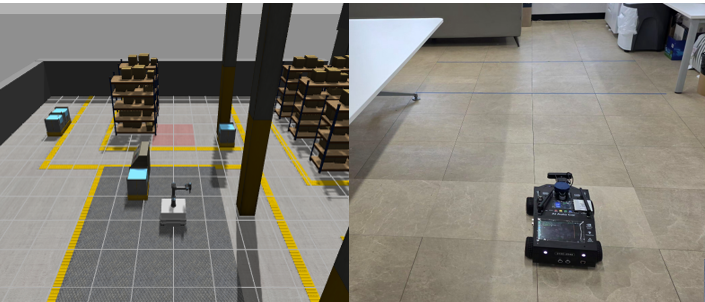
\includegraphics[width=\columnwidth]{fig_env.png}
\vspace{-2ex}
\caption{Experimental environments. \textbf{Left:} Gazebo warehouse simulation with red-outlined forbidden zones. \textbf{Right:} Real Jetson Nano Ackermann-steering robot used for physical validation with blue-outlined forbidden zones.}
\label{fig:env}
\end{figure}

\begin{table}[t]
\centering
\tblstyle
\caption{Confusion matrix --- Gazebo simulation (S1--S4, 20 seeds). Within-margin probes are reported separately (Table~\ref{tab:probes}), so no method incurs a true false positive.}
\label{tab:confusion}
\footnotesize
\begin{tabular}{@{}l rrr rrrr@{}}
\toprule
& \multicolumn{3}{c}{Trial Counts} & \multicolumn{4}{c}{Confusion Matrix} \\
\cmidrule(lr){2-4} \cmidrule(lr){5-8}
Method & $N$ & Valid & Infra & TP$\uparrow$ & FP$\downarrow$ & TN$\uparrow$ & FN$\downarrow$ \\
\midrule
No Guard & 300 & 256 & 4 & 0 & 0 & 59 & 197 \\
SELP & 300 & 259 & 1 & 20 & 0 & 60 & 179 \\
CBF & 300 & 260 & 0 & 23 & 0 & 60 & 177 \\
SSM & 300 & 260 & 0 & 22 & 0 & 60 & 178 \\
RoboGuard & 300 & 260 & 0 & 20 & 0 & 60 & 180 \\
CBF-Adaptive & 300 & 260 & 0 & 84 & 0 & 60 & 116 \\
\rowcolor{lightgray} \textbf{PETSE (Ours)} & 300 & 260 & 0 & \textbf{200} & \textbf{0} & 60 & \textbf{0} \\
\bottomrule
\end{tabular}
\end{table}

\begin{table}[t]
\centering
\tblstyle
\caption{Detection performance with 95\,\% confidence intervals (Wilson score for recall; bootstrap, 2000 resamples, for F1). Precision is $1.000$ for every method because within-margin probes are excluded from the confusion matrix (Table~\ref{tab:probes}).}
\label{tab:detection}
\footnotesize
\begin{tabular}{@{}l c c c@{}}
\toprule
Method & Recall [95\,\% CI]$\uparrow$ & F1 [95\,\% CI]$\uparrow$ & FNR$\downarrow$ \\
\midrule
No Guard & 0.000 [0.000, 0.019] & 0.000 [0.000, 0.000] & 100.0\% \\
SELP & 0.101 [0.066, 0.150] & 0.183 [0.115, 0.249] & 89.9\% \\
CBF & 0.115 [0.078, 0.167] & 0.206 [0.137, 0.276] & 88.5\% \\
SSM & 0.110 [0.074, 0.161] & 0.198 [0.130, 0.267] & 89.0\% \\
RoboGuard & 0.100 [0.066, 0.149] & 0.182 [0.113, 0.251] & 90.0\% \\
CBF-Adaptive & 0.420 [0.354, 0.489] & 0.592 [0.520, 0.658] & 58.0\% \\
\rowcolor{lightgray} \textbf{PETSE (Ours)} & \textbf{1.000 [0.981, 1.000]} & \textbf{1.000 [1.000, 1.000]} & \textbf{0.0\%} \\
\bottomrule
\end{tabular}
\end{table}

\begin{table}[t]
\centering
\tblstyle
\caption{Violation rate (VR, \%): fraction of valid trials resulting in physical zone entry ($\text{VR} = n_{\text{violated}} / n_{\text{valid}}$, within-margin probes included). Per-scenario columns report within-scenario rates. Lower is better. PETSE records $0$ violations in $300$ trials (rule-of-three 95\,\% upper bound $\le 1.0\%$).}
\label{tab:vr}
\footnotesize
\begin{tabular}{@{}l ccccc@{}}
\toprule
Method & Overall & S1 & S2 & S3 & S4 \\
\midrule
No Guard              & 66.7 & 39.8 &  75.3 & 100.0 & 74.7 \\
SELP                  & 58.6 & 19.6 &  75.0 &  90.0 & 73.8 \\
CBF                   & 56.0 & 19.0 &  71.2 &  90.0 & 70.0 \\
SSM                   & 56.7 & 19.0 &  71.2 &  87.5 & 73.8 \\
RoboGuard             & 57.0 & 20.0 &  72.5 &  90.0 & 71.2 \\
CBF-Adaptive          & 34.0 & 19.0 &  70.0 &  57.5 &  5.0 \\
\rowcolor{lightgray} \textbf{PETSE (Ours)} & \textbf{0.0} & \textbf{0.0} &
\textbf{0.0} & \textbf{0.0} & \textbf{0.0} \\
\bottomrule
\end{tabular}
\end{table}

\begin{table}[t]
\centering
\tblstyle
\caption{Within-margin probe rejections (designed conservatism, not false positives). Probes sit outside the zone but inside PETSE's $0.562$\,m margin. A method rejects a probe iff the probe lies inside its own margin; the staircase is the margin formula acting as designed. ($^{*}$RoboGuard uses a fixed buffer smaller than the probe distances.)}
\label{tab:probes}
\footnotesize
\begin{tabular}{@{}l c cc@{}}
\toprule
Method & Margin (m) & near (0.15\,m) & mid (0.45\,m) \\
\midrule
No Guard & 0 & 0/19 & 0/19 \\
SELP & 0 & 0/19 & 0/19 \\
CBF & 0.30 & 20/20 & 0/20 \\
SSM & 0.575 & 20/20 & 20/20 \\
RoboGuard & 0$^{*}$ & 0/20 & 0/20 \\
CBF-Adaptive & 0.562 & 20/20 & 20/20 \\
\rowcolor{lightgray} \textbf{PETSE (Ours)} & 0.562 & 20/20 & 20/20 \\
\bottomrule
\end{tabular}
\end{table}

\begin{table}[t]
\centering
\tblstyle
\caption{Paired significance --- PETSE vs.\ each baseline (exact McNemar, detection success on unsafe trials, paired by scenario/intensity/seed). ``PETSE\,$\checkmark$'' and ``Base\,$\checkmark$'' count discordant pairs. No pair favors any baseline; all $p$ survive Holm correction. Last column: per-seed recall (mean\,$\pm$\,SD, 20 seeds).}
\label{tab:mcnemar}
\footnotesize
\begin{tabular}{@{}l c cc c c@{}}
\toprule
Baseline & Pairs & PETSE\,$\checkmark$ & Base\,$\checkmark$ & Holm $p$ & Recall (seed) \\
\midrule
No Guard & 197 & 197 & 0 & $<0.001$ & $0.000\pm0.000$ \\
SELP & 199 & 179 & 0 & $<0.001$ & $0.101\pm0.002$ \\
CBF & 200 & 177 & 0 & $<0.001$ & $0.115\pm0.037$ \\
SSM & 200 & 178 & 0 & $<0.001$ & $0.110\pm0.031$ \\
RoboGuard & 200 & 180 & 0 & $<0.001$ & $0.100\pm0.000$ \\
CBF-Adaptive & 200 & 116 & 0 & $<0.001$ & $0.420\pm0.111$ \\
\rowcolor{lightgray} \textbf{PETSE} & --- & --- & --- & --- & $\mathbf{1.000\pm0.000}$ \\
\bottomrule
\end{tabular}
\end{table}

Table~\ref{tab:confusion} aggregates confusion-matrix counts over four attack scenarios (infrastructure failures and within-margin probes excluded; the latter are reported in Table~\ref{tab:probes}). Each method runs 300 trials over 20 seeds; after separating 40 within-margin probes, the confusion matrix spans 200 attack trials whose goals or paths target the forbidden zone and 60 safe trials. Without protection (No Guard) every valid attack trial ends in zone entry (TP\,=\,0). The strongest baseline, CBF-Adaptive, reaches only TP\,=\,84 with FN\,=\,116, and no other baseline exceeds TP\,=\,23. PETSE blocks every unsafe trial (TP\,=\,200, FN\,=\,0) and, because near/mid-boundary rejections are accounted separately as designed conservatism (Table~\ref{tab:probes}), incurs no false positive (FP\,=\,0)---as do all baselines under this accounting.

Table~\ref{tab:detection} confirms the gap: the best baseline recall is $0.420$ (CBF-Adaptive, FNR\,=\,58\,\%), whereas PETSE attains recall $1.000$ [0.981, 1.000] and F1 $1.000$ with zero false negatives; its confidence intervals do not overlap those of any baseline. The paired significance tests (Table~\ref{tab:mcnemar}) confirm the gap is not a seed artifact: PETSE strictly dominates every baseline (exact McNemar $p<0.001$ after Holm correction, with zero discordant pairs favoring any baseline), and its per-seed recall is $1.000\pm0.000$.

Table~\ref{tab:vr} reports the violation rate (VR), the fraction of valid trials that end in physical zone entry (within-margin probes included in the denominator). Every baseline leaves $34$--$67\%$ of trials violating---even CBF-Adaptive, which uses PETSE's exact margin---whereas PETSE records $0.0\%$ in all four scenarios ($0$ of $300$ trials; rule-of-three 95\,\% upper bound $\le 1.0\%$).

\textbf{S1 (Direct Hazard Goal).} Baselines allow 19.0--39.8\,\% violations because goal-level approval alone cannot absorb execution-time uncertainty. PETSE's goal gate blocks every hazardous coordinate (VR\,=\,0.0\,\%).

\textbf{S2 (Implicit Path Inducement).} No Guard (75.3\,\%), SELP (75.0\,\%), CBF (71.2\,\%), SSM (71.2\,\%), RoboGuard (72.5\,\%), and CBF-Adaptive (70.0\,\%) all remain near the unprotected rate, since none inspects path geometry when the goal itself lies outside the zone. PETSE's segment--polygon intersection test against the inflated boundary yields VR\,=\,0.0\,\%.

\textbf{S3 (Velocity Manipulation + Delay).} Covert velocity amplification produces cumulative overshoot that control-layer methods cannot absorb; CBF-Adaptive still records VR\,=\,57.5\,\%. PETSE's per-cycle distance check, combined with its velocity-aware margin, keeps VR at 0.0\,\%.

\textbf{S4 (Position Spoofing).} SELP (73.8\,\%) and SSM (73.8\,\%) stay close to No Guard (74.7\,\%); CBF (70.0\,\%) and RoboGuard (71.2\,\%) improve only marginally. CBF-Adaptive blocks most spoofing (VR\,=\,5.0\,\%) thanks to its enlarged margin, but PETSE eliminates all residual failures (VR\,=\,0.0\,\%) by coupling the covariance-based margin with continuous position monitoring---the mechanism isolated causally in Section~\ref{sec:reverify}.

\textbf{Why the non-adaptive baselines cluster.} SELP, CBF, SSM, and RoboGuard
sit within a few points of one another in every scenario (Overall $56$--$59\%$)
not because they are implemented alike but because they share a single blind
spot: none re-verifies the \emph{path} or the \emph{execution-time} state.
SELP and RoboGuard are action-level checkers---each rejects only a goal
\emph{coordinate} that lies inside a zone, with no geometric margin and no
path test---so on our fixed-zone scenarios they return identical decisions by
construction (we confirmed this by running RoboGuard's own LTL/B\"uchi
implementation: $0$ decision differences over an $836$-goal grid). CBF and SSM
add only a small point-margin ($0.30$ and $0.575$\,m) that rarely changes the
outcome once the goal sits outside the zone. Consequently all four fail on the
same post-approval trials---most visibly in S2, where the goal is safe but the
path is not. The lone baseline that breaks from the cluster is CBF-Adaptive
($34\%$ overall, S4 VR\,$=5.0\%$), and it does so precisely by adopting PETSE's
covariance-based margin. The discriminating factor is therefore not the method
family but whether a defense (i)~inflates the margin to the localization
uncertainty and (ii)~re-verifies at execution time---exactly the two
ingredients PETSE combines.

\subsection{CBF-Adaptive vs. PETSE}
Although both methods inflate the margin by the same magnitude, three architectural differences explain the performance gap.

\textbf{Dynamics-model dependency.} CBF requires a dynamics model $\dot{x}=f(x)+g(x)u$ and solves a QP for safe inputs; model inaccuracy invalidates the safe set. PETSE checks only a geometric distance condition $\mathrm{dist}(\hat{p}_t,\mathcal{F})\ge M(t)$ and needs no dynamics model at all.

\textbf{Inside vs.\ outside the control loop.} CBF modifies the control input $u$ \emph{inside} the loop, so a compromised control channel (S3) can prevent the safe input from reaching the actuator (CBF-Adaptive S3: VR\,=\,57.5\,\%). PETSE monitors position \emph{outside} the loop and intervenes by cancelling the goal or commanding a stop, operating independently of the nominal controller output while relying on the trusted stop channel (S3: VR\,=\,0.0\,\%).

\textbf{Path-level verification.} CBF constrains instantaneous control but never inspects whether the \emph{planned trajectory} traverses a forbidden zone. In S2, CBF-Adaptive's VR reaches 93.3\,\%---nearly identical to No Guard (100.0\,\%). PETSE rejects the path at the goal gate before motion begins (S2: VR\,=\,0.0\,\%).

\subsection{Runtime Re-Verification Closes the Post-Approval Attack Surface}\label{sec:reverify}

The comparison above varies the architecture; here we hold the architecture fixed and vary only the runtime monitor, to test our central claim directly: post-approval safety comes from continuous re-verification, not from the margin width. We use the position-spoofing scenario (S4) as a time-of-check to time-of-use (TOCTOU) attack, in which a localization bias $\Delta$ is injected \emph{only} during the planning window---so the goal gate approves a path computed from a biased pose---and removed before motion, so the robot executes the true, unsafe path. The biased path-$y$ at the zone is $0.914 + \frac{3}{7}\Delta$; the goal gate approves once it exceeds the margin boundary $y^\star{=}1.389$\,m, i.e., for $\Delta{>}\Delta^\star{\approx}1.11$.

\textbf{Paired factorial (margin fixed).} We run a $2{\times}2$ design over 10 seeds with the margin fixed at $0.562$\,m: \{monitor OFF, ON\}~$\times$~\{$\Delta$ below, above $\Delta^\star$\}. Below the boundary the goal gate rejects the task pre-motion regardless of the monitor (violation $0/10$ in both arms). Above the boundary the attack defeats the goal gate; with the monitor OFF---check-once approval---all ten trials enter the zone ($10/10$ violated), whereas with the monitor ON all ten are stopped ($0/10$: seven by explicit runtime rejection, three by continuous command-shaping that steers the footprint around the zone). The ten seed-paired trials are all discordant in the monitor's favor (exact McNemar $p{=}1.95{\times}10^{-3}$). Since the margin is identical in both arms, the $100\%{\rightarrow}0\%$ swing is attributable to the runtime monitor alone (Fig.~\ref{fig:toctou}(a)).

\textbf{Boundary characterization.} Sweeping $\Delta$ with the monitor OFF (Fig.~\ref{fig:toctou}(b)), the violation rate steps from $0/10$ at biased-$y{=}1.386$\,m to $10/10$ at $1.429$\,m, bracketing the analytically predicted boundary $y^\star{=}1.389$\,m. The empirical transition coincides with the goal-gate margin, confirming that the above/below conditions are not hand-tuned.

\textbf{Controller-agnostic.} The runtime monitor acts on the command channel, below any local planner. Repeating the $2{\times}2$ under a structurally different Nav2 controller---Regulated Pure Pursuit (RPP) instead of DWB, speed matched at $0.22$\,m/s---reproduces the result exactly: attack surface $10/10$ with the monitor OFF and $0/10$ with it ON, for both controllers (Fig.~\ref{fig:ctrlgen}). The guarantee is therefore an execution-layer property, not an artifact of a particular planner.

\textbf{Operating point.} Continuous checking raises two concerns---nuisance stops and late reaction---that we address from the full campaign (Fig.~\ref{fig:oppoint}). Across 243 benign trajectories the monitor never triggered a spurious mid-execution abort ($0$ aborts; rule-of-three upper bound $\le 1.23\%$), and all 60 clearly-safe goals completed. Across all 55 runtime interventions the robot never entered the zone; each stop retained positive clearance---median $3.12$\,m for velocity/deviation attacks (caught early) and $0.45$\,m for the harder TOCTOU case, worst case $0.066$\,m---at a median reaction latency of $50$\,ms.

\begin{figure*}[t]
    \centering
    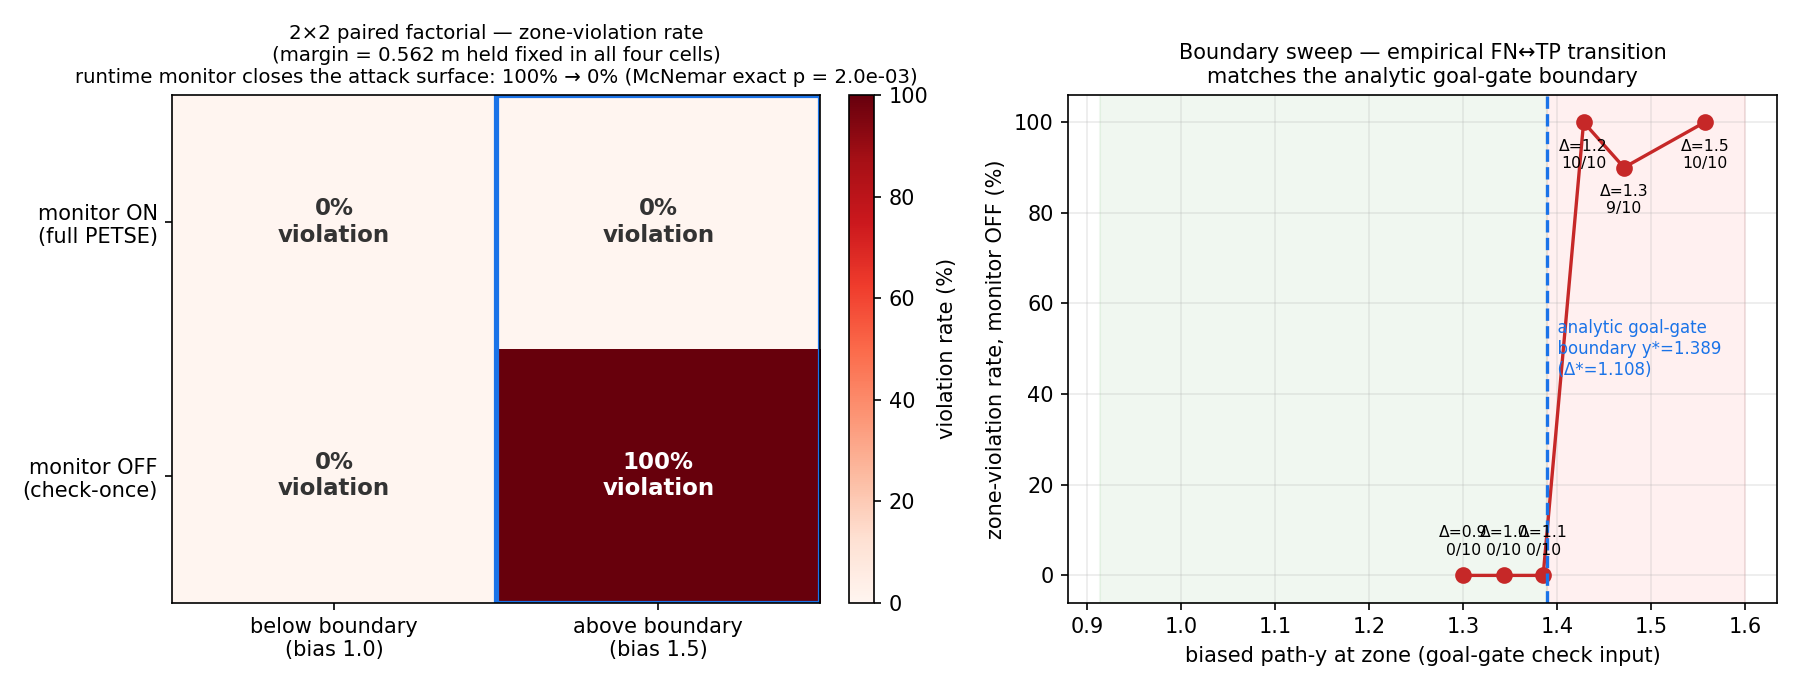
\includegraphics[width=0.98\textwidth]{toctou_ablation.png}
    \vspace{-1ex}
    \caption{Runtime re-verification with the margin held fixed at $0.562$\,m. \textbf{(a)}~$2{\times}2$ paired factorial: only the (monitor~OFF, above-boundary) cell violates ($100\%$); enabling the monitor drives it to $0\%$ (exact McNemar $p{=}1.95{\times}10^{-3}$). \textbf{(b)}~Boundary sweep (monitor OFF): the empirical $\text{FN}{\leftrightarrow}\text{TP}$ transition matches the analytic goal-gate boundary $y^\star{=}1.389$\,m.}
    \label{fig:toctou}
\end{figure*}

\begin{figure*}[t]
    \centering
    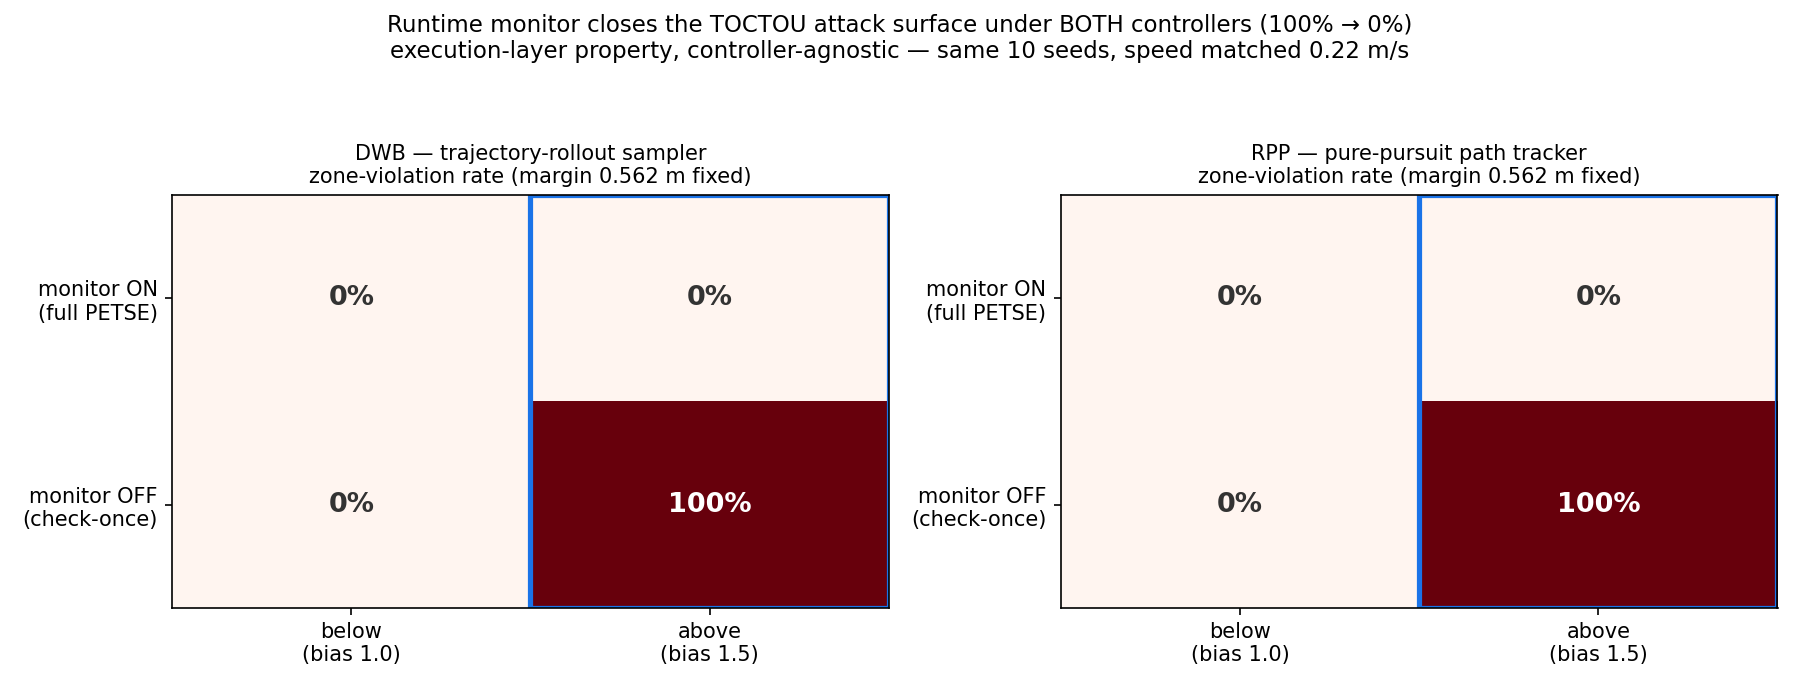
\includegraphics[width=0.98\textwidth]{controller_generalization.png}
    \vspace{-1ex}
    \caption{Controller generalization. The same S4 TOCTOU $2{\times}2$ under DWB (trajectory-rollout sampler) and RPP (pure-pursuit tracker), speed matched. The monitor closes the attack surface ($100\%{\rightarrow}0\%$) identically under both, confirming an execution-layer, controller-agnostic property.}
    \label{fig:ctrlgen}
\end{figure*}

\begin{figure*}[t]
    \centering
    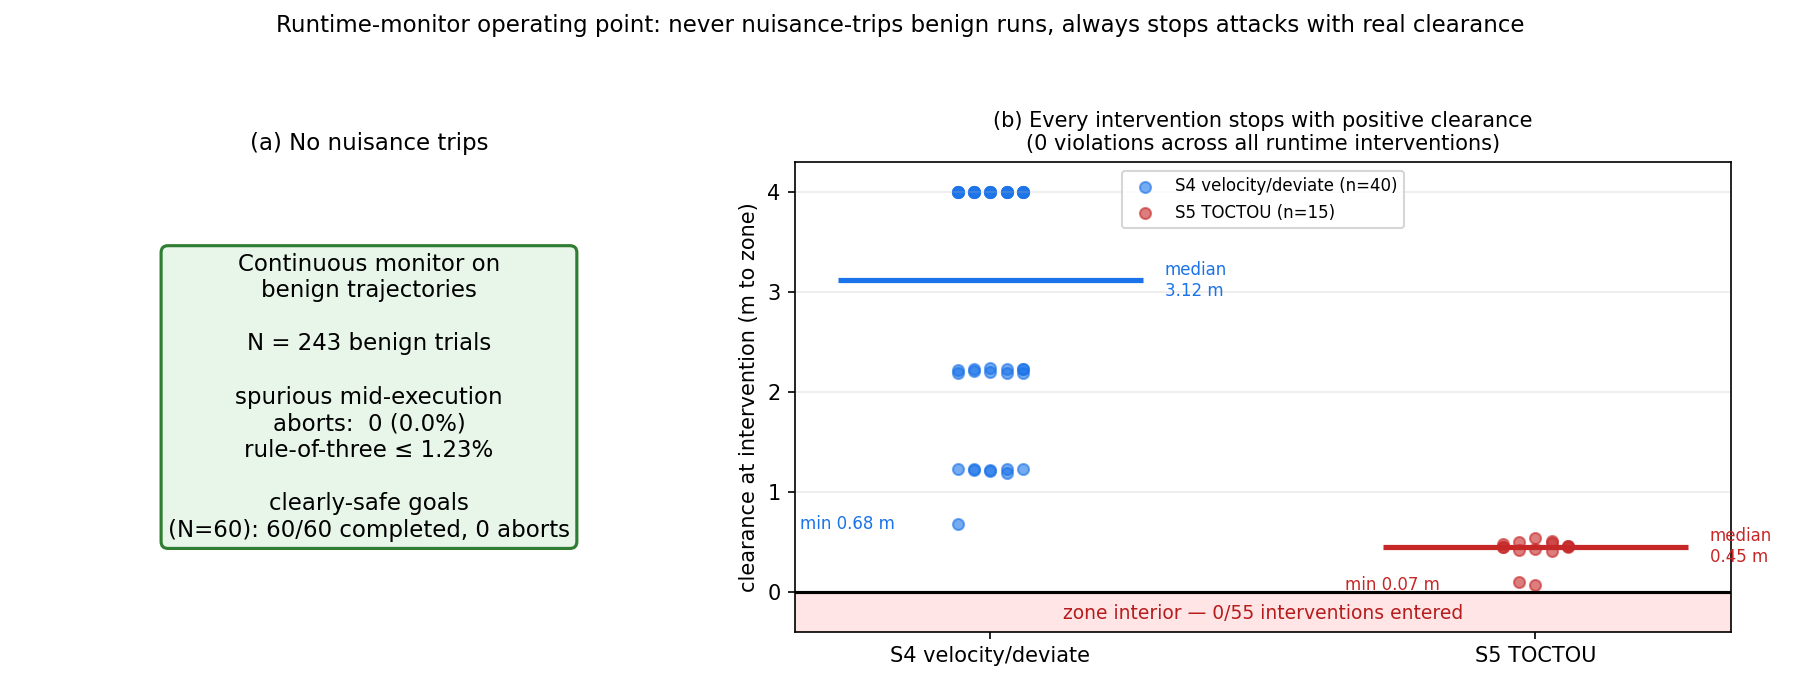
\includegraphics[width=0.98\textwidth]{monitor_operating_point.png}
    \vspace{-1ex}
    \caption{Runtime-monitor operating point. \textbf{(a)}~No nuisance trips: $0/243$ benign trajectories aborted mid-execution. \textbf{(b)}~Every one of the 55 interventions stops with positive clearance to the zone ($0$ violations); velocity/deviation attacks are caught early (median $3.12$\,m), TOCTOU near the boundary (median $0.45$\,m).}
    \label{fig:oppoint}
\end{figure*}

\subsection{Execution-Time-Only Attacks: Hijack and Time-Varying Zones}\label{sec:exectime}
Two scenarios (S5, S6) isolate attacks that succeed \emph{only} after approval, where prompt- and planning-stage defenses are structurally blind; each runs five seeds per method on the warehouse map.

\textbf{S5 (Localization-spoofing hijack).} An approved, clean-pose goal is followed by map-consistent LiDAR spoofing that biases $\hat p_t$ away from the confidential zone while the true robot drives in. Every planning-layer baseline is defeated (Fig.~\ref{fig:hijack}): No~Guard, SELP, and CBF-inflated each enter the zone in all $5/5$ trials (mean $89$--$179$ in-zone samples), because none re-checks the constraint against an independent channel once motion is approved---CBF simply trusts the spoofed pose it is handed. PETSE enters in $0/5$: its runtime cross-check of the exteroceptive estimate against the proprioceptive odometry (Section~\ref{sec:threat_model}) detects the growing disagreement and fail-stops. This is the paper's central security result---an execution-layer, cross-channel monitor is the only defense that survives post-approval sensor spoofing.

\begin{figure}[t]
    \centering
    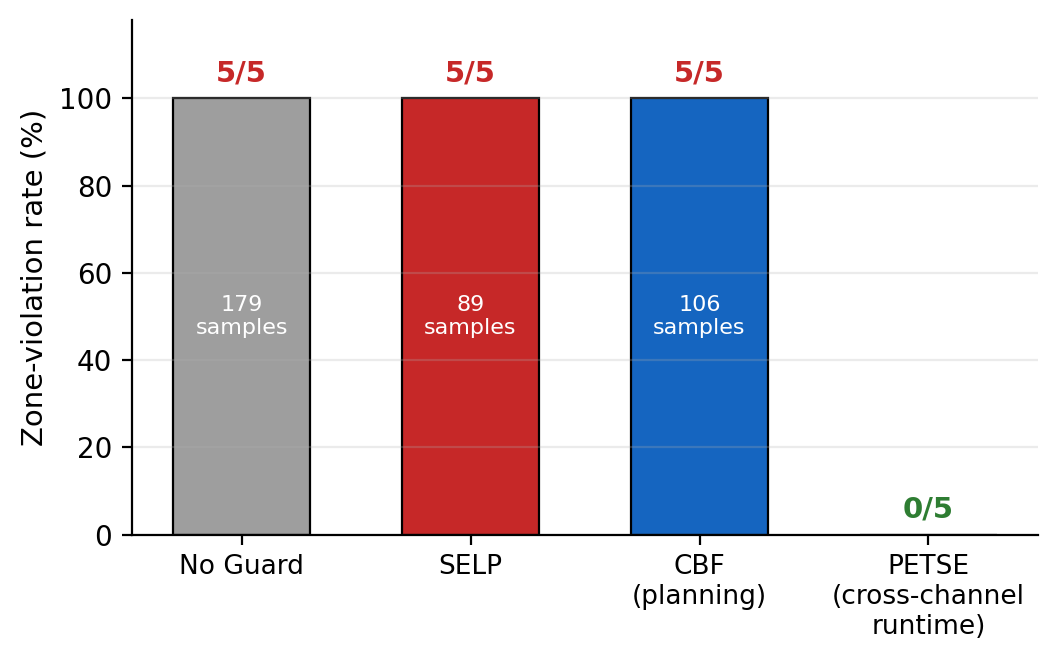
\includegraphics[width=0.82\linewidth]{fig_hijack.png}
    \vspace{-1.0ex}
    \caption{S5 localization-spoofing hijack (warehouse, five seeds). Map-consistent LiDAR spoofing after goal approval defeats every planning-layer baseline ($5/5$ zone entries); only PETSE's cross-channel runtime re-verification holds ($0/5$).}
    \label{fig:hijack}
\end{figure}

\textbf{S6 (Time-varying zone).} A goal is approved on a clear path; a keep-out region is then activated mid-navigation. Approval-time-only methods (No~Guard, SELP) drive straight in ($5/5$), whereas \emph{any} continuous re-verifier stops before entry---both PETSE and a guard-equipped CBF achieve $0/5$. Unlike S5, S6 involves no spoofing, so a runtime monitor alone suffices and no cross-channel anchor is needed. The contrast sharpens the claim: continuous re-verification is necessary for both, but sensor-spoofing attacks (S5) additionally demand the cross-channel check that distinguishes PETSE from a merely runtime-monitored CBF.


\subsection{Ablation Study}\label{sec:ablation}

Robustness is stress-tested with a 1D kinematic model under injected uncertainty. In one dimension the estimation term simplifies to $z_{1-\varepsilon}\,\sigma$, giving
\begin{equation}
M = z_{1-\varepsilon}\,\sigma + (e_0 + c_1 v) + v\tau + \frac{v^2}{2a_{\max}}.
\end{equation}

Fig.~\ref{fig:stress} sweeps uncertainty up to $10\times$ the nominal level. A fixed margin breaks down rapidly (VR up to 41.9\,\%), while the adaptive formulation keeps VR\,$\le$\,0.3\,\% throughout, confirming that the margin scales proportionally to uncertainty. The risk parameter $\varepsilon$ governs the resulting safety--availability trade-off.

\begin{figure}[t]
    \centering
    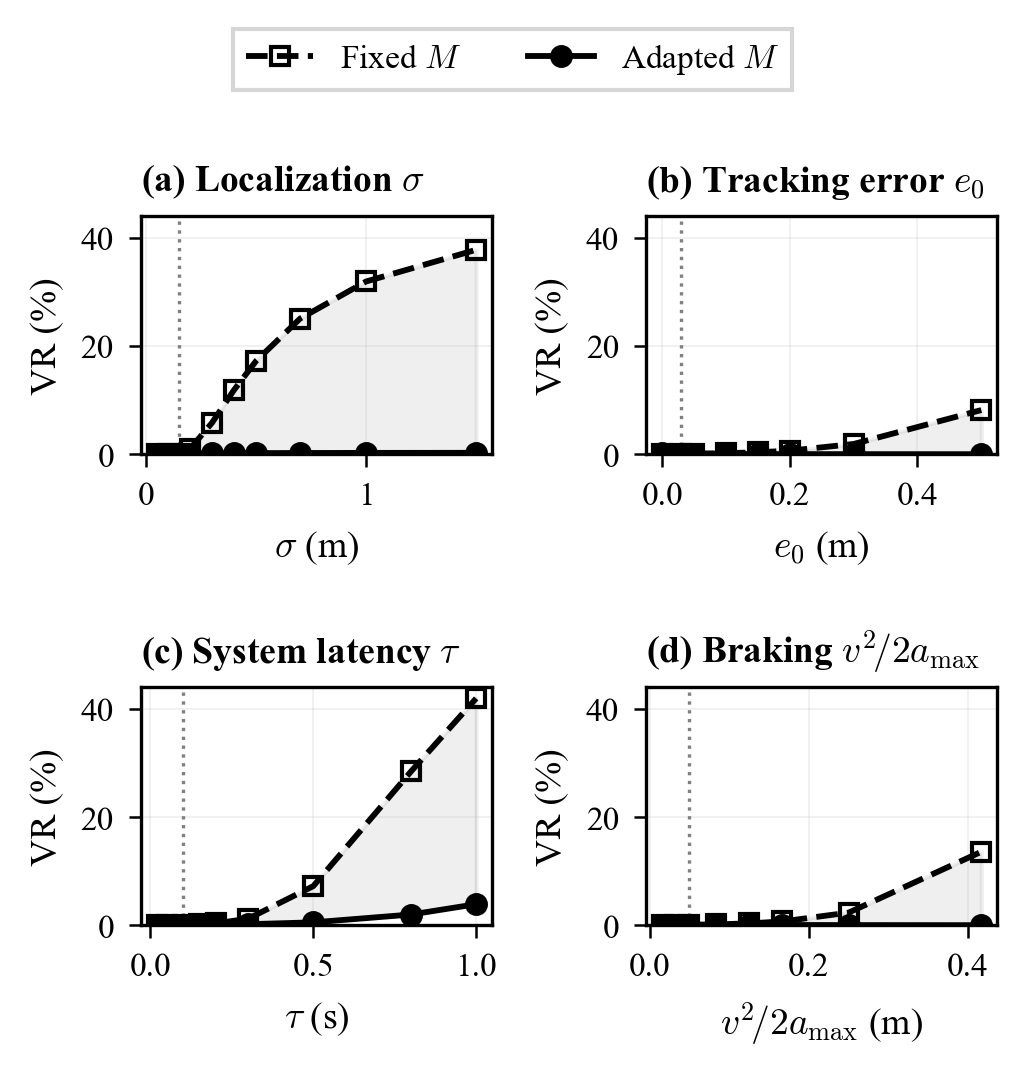
\includegraphics[width=0.95\linewidth]{fig_stress_test.png}
    \vspace{-1.5ex}
    \caption{Violation rate under increasing uncertainty. Dashed: fixed margin; solid: adaptive margin.}
    \label{fig:stress}
\end{figure}

\subsection{Assumption Violation Under a Full-Stack Over-Speed Attack}\label{sec:velreact}
The 1D sweep abstracts the platform away. To confirm that the same failure mode appears in the full Gazebo stack---and to isolate \emph{why} a fixed margin is unsafe---we compare against a \emph{reactive fixed-margin} baseline: a costmap-inflation-style buffer~\cite{lu2014layered} that stops the robot only once its \emph{current} position falls within a fixed $0.55$\,m of the zone, with no velocity-adaptive re-verification. This baseline trusts the declared velocity bound $v_{\max}{=}0.5$\,m/s: a buffer sized for that bound suffices only if the robot never exceeds it. An attacker who has gained the ability to publish \texttt{cmd\_vel} (Section~\ref{sec:threat_model}) violates exactly that assumption, injecting a straight-line command that drives the robot toward the zone at the platform ceiling of $1.5$\,m/s ($3\times$ the declared bound). Because the reactive buffer only reacts at the trigger distance, the true braking distance at $3\times$ speed exceeds it and the robot overshoots.

Fig.~\ref{fig:velreact} reports the minimum clearance to the zone over five seeds per method. The reactive fixed-margin baseline breaches its own $0.55$\,m safety margin in \emph{all} five seeds (clearance collapsing to $0.00$--$0.29$\,m: the vehicle body---radius ${\approx}0.25$\,m---is already inside the forbidden polygon, and its centroid crosses the boundary in $2/5$ seeds), statistically indistinguishable from having no guard at all ($5/5$ breach). PETSE, which re-verifies the distance constraint every control cycle against a margin recomputed from the \emph{measured} velocity rather than the declared one, retains a $2.15$--$2.22$\,m clearance and never approaches the margin ($0/5$ breach). The vulnerability is thus specific to trusting a declared velocity bound; continuous re-verification with an online velocity estimate removes it, corroborating the 1D result in the full sensorimotor loop.

\begin{figure}[t]
    \centering
    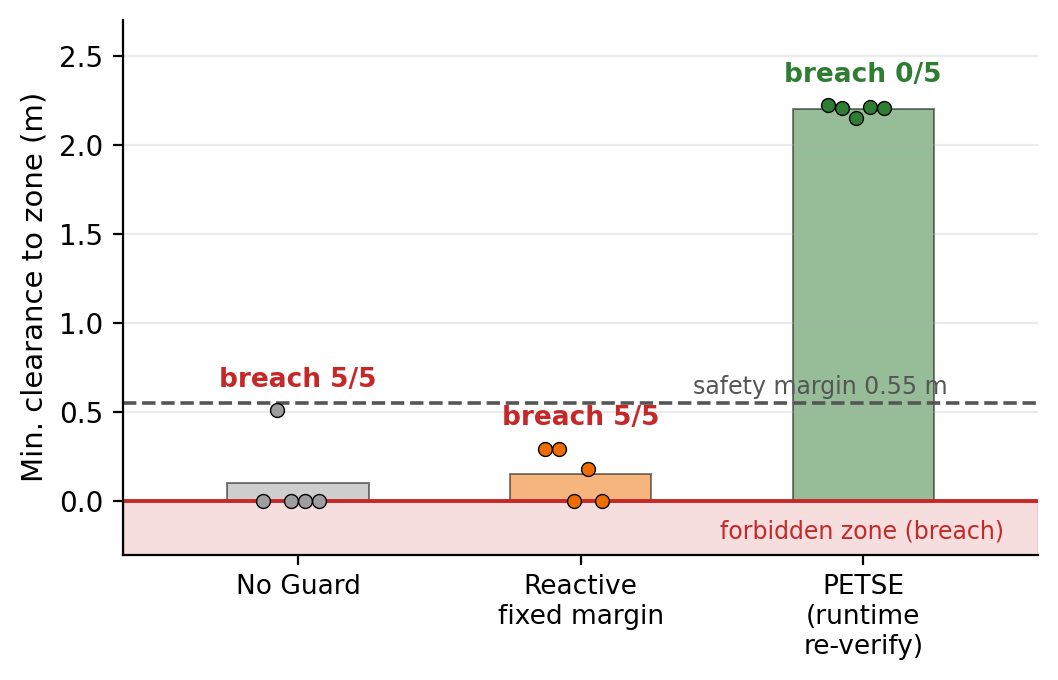
\includegraphics[width=0.9\linewidth]{fig_velocity_reactive.png}
    \vspace{-1.0ex}
    \caption{Assumption violation (velocity bound), full Gazebo stack: minimum clearance to the zone under a $3\times$ over-speed \texttt{cmd\_vel} injection (five seeds each; dots are per-seed, bars are the mean). A reactive fixed margin that trusts the declared $v_{\max}$ breaches its own $0.55$\,m safety margin in every seed (clearance $\le0.29$\,m; body inside the zone), whereas PETSE's velocity-adaptive re-verification holds ${\approx}2.2$\,m clearance.}
    \label{fig:velreact}
\end{figure}

\subsection{Real-Robot Validation}\label{sec:real}
A total of 140 real-robot trials were conducted (20 per condition: PETSE in all four scenarios, No Guard in B--D) on a Jetson Nano Ackermann-steering car ($v_{\max}{=}0.1$\,m/s, $a_{\max}{=}1.5$\,m/s$^2$) that relies on dead-reckoning odometry rather than AMCL. Because no particle-filter covariance is available, $M_{\mathrm{est}}$ is instead set to $z_{1-\varepsilon}\,\sigma$ with a fixed $\sigma{=}0.15$\,m (the 1D reduction of Section~\ref{sec:ablation}), showing that the framework accepts any position-uncertainty estimate, not only AMCL output. The forbidden zone is an annulus centered at the origin (inner radius 3.0\,m, outer 3.9\,m). With $\varepsilon{=}0.003$, $e_0{=}0.03$\,m, $c_1{=}0.04$\,s, and $\tau{=}0.2$\,s, the resulting margin is $M{\approx}0.47$\,m---smaller than the simulation value ($0.562$\,m) because the lower platform speed shrinks both the latency-drift and braking-distance terms. The PETSE algorithm is otherwise identical; only platform-specific observables change. Although the trial count is modest, outcomes are deterministic across all 140 runs and consistent with the simulation trends.

\textbf{Scenario A (Safe Goal).} Goal $(0,\,1.5)$\,m lies well outside the zone. PETSE issued ALLOW in every trial; the robot reached its target with no violations (mean stop distance $1.39\pm0.03$\,m from the origin).

\textbf{Scenario B (S2---Implicit Path).} Goal $(0,\,5.8)$\,m is safe, but the straight-line path cuts through the annulus. The goal gate passed it, yet the runtime monitor detected $\mathrm{dist}(\hat{p}_t, \mathcal{F}) < M(t)$ mid-execution and triggered an emergency stop at a mean distance of $2.53\pm0.02$\,m, preserving a ${\approx}0.47$\,m gap to the inner zone wall---matching $M$. Without PETSE, all 20 trials crossed the zone (mean $4.82\pm0.31$\,m).

\textbf{Scenario C (S3---Velocity Manipulation).} Goal $(0,\,2.0)$\,m was approved, but execution velocity was amplified $1.5\times$. Unprotected, the robot overshot into the zone in every trial (mean $4.59\pm0.79$\,m). With PETSE, the distance monitor fired an emergency stop in all 20 trials before zone entry (mean $1.80\pm0.57$\,m).

\textbf{Scenario D (S4---Position Spoofing).} A 0.5\,m static offset ($\sigma_{\mathrm{spoof}}{=}0.01$) was added to the pose estimate while the robot headed toward a safe goal. Without PETSE, the spoofed estimate hid the true approach and violations occurred in all 20 runs (mean $4.55\pm0.24$\,m). PETSE's covariance-based margin absorbed the offset and the monitor stopped the robot in every trial (mean $1.62\pm0.91$\,m).

\begin{table}[t]
\centering
\tblstyle
\caption{Real-robot validation results (140 trials).}
\label{tab:real}
\footnotesize
\begin{tabular}{@{}l l ccccc@{}}
\toprule
Scenario & Guard & Trials & Decision & \makecell{Zone\\Viol.} & \makecell{Mean Stop\\Dist.\,(m)} & Std\,(m) \\
\midrule
A: Safe Goal & PETSE & 20 & ALLOW & 0/20 & 1.39 & 0.03 \\
B: S2 & PETSE & 20 & PATH\_STOP & 0/20 & 2.53 & 0.02 \\
B: S2 & No Guard & 20 & --- & 20/20 & 4.82 & 0.31 \\
\midrule
C: S3 & PETSE & 20 & E\_STOP & 0/20 & 1.80 & 0.57 \\
C: S3 & No Guard & 20 & --- & 20/20 & 4.59 & 0.79 \\
D: S4 & PETSE & 20 & E\_STOP & 0/20 & 1.62 & 0.91 \\
D: S4 & No Guard & 20 & --- & 20/20 & 4.55 & 0.24 \\
\bottomrule
\end{tabular}
\end{table}

Table~\ref{tab:real} summarizes the outcomes. PETSE made the correct decision in every PETSE-enabled trial: safe goals were allowed (Scenario~A) and all attacks were stopped before zone entry (B--D). No Guard produced 20/20 violations in each attack scenario. The measured safety gap (${\approx}0.47$\,m) matches the formula-predicted margin on a platform whose dynamics and sensors differ from the simulation, and the deterministic 0/20 vs.\ 20/20 separation across four conditions provides clear evidence of cross-platform transfer. The 1{,}920-trial simulation study supplies the corresponding statistical power.

\subsection{Attack-Surface Boundary: Coordinated Dual-Channel Spoofing}\label{sec:coord}
The results above hold under Assumption~A1 (Section~\ref{sec:threat_model}), i.e., an
honest proprioceptive channel. We now deliberately \emph{violate} A1 to map the exact
boundary of PETSE's guarantee against the strongest---and out-of-scope---adversary: one
that spoofs both channels at once. A LiDAR spoof displaces $\hat{p}_t$ to lure the true
robot toward $F$, while a synchronized odometry spoof drives $o_t$ to follow $\hat{p}_t$,
holding the cross-channel residual $\varepsilon=\lVert \hat{p}_t-o_t\rVert$ near a
controlled value. PETSE's consistency check fires only when this residual exceeds a
threshold $\tau_c$ set from the benign offset distribution ($\tau_c{=}0.95$\,m here); the
adversary's task is thus to keep the observed residual below $\tau_c$. We sweep the target
$\varepsilon\in\{0,0.3,0.6,0.8,0.95,1.1,1.3\}$\,m (three seeds each) under CUSUM enforcement
and score, per level, whether the robot is halted \emph{before} $F$ (defense holds) or
enters it (defense evaded).

Protection degrades \emph{gracefully} rather than at a knife edge (Fig.~\ref{fig:coord}).
Under perfect coordination ($\varepsilon{=}0$) the residual stays near zero, the monitor is
blind, and every effective lure reaches $F$ (3/3 incursions)---PETSE is fully defeated. The
incursion rate then falls with $\varepsilon$ and vanishes once the \emph{observed} residual
crosses $\tau_c$, which occurs around $\varepsilon{\approx}0.8$\,m: no trial incurs for
$\varepsilon\ge0.95$\,m. The transition is soft because two effects compound. First,
real-time dual-channel coordination is imperfect: the observed residual equals the target
plus a tracking error of $0.2$--$0.3$\,m (e.g., a nominal $\varepsilon{=}0.8$ yields an
observed $d_{\mathrm{abs}}$ of $0.98$--$1.02$), so the attacker must aim for a target
$\varepsilon\lesssim0.65$ to keep the residual below $\tau_c$. Second, once the residual
does cross $\tau_c$ the fail-stop still races the robot to $F$, so a late crossing
occasionally permits entry. The upshot is a quantified coordination burden: to evade PETSE
the adversary must not merely spoof the exteroceptive LiDAR (scenario S4) but also drive
on-board odometry to agree with it, in real time, to a residual well below $\tau_c$---which,
per~A1, presupposes compromise of the on-board compute. Below that capability, single-channel
spoofing is caught, consistent with the $0.0\%$ violation rate of
Section~\ref{sec:experiments}. Tightening $\tau_c$ shrinks the evasion window but trades off
benign false alarms (Section~\ref{sec:reverify}); the residual privileged-adversary risk is
instead the province of the independent hardware safety channel of
Section~\ref{sec:threat_model}.

\begin{figure}[t]
    \centering
    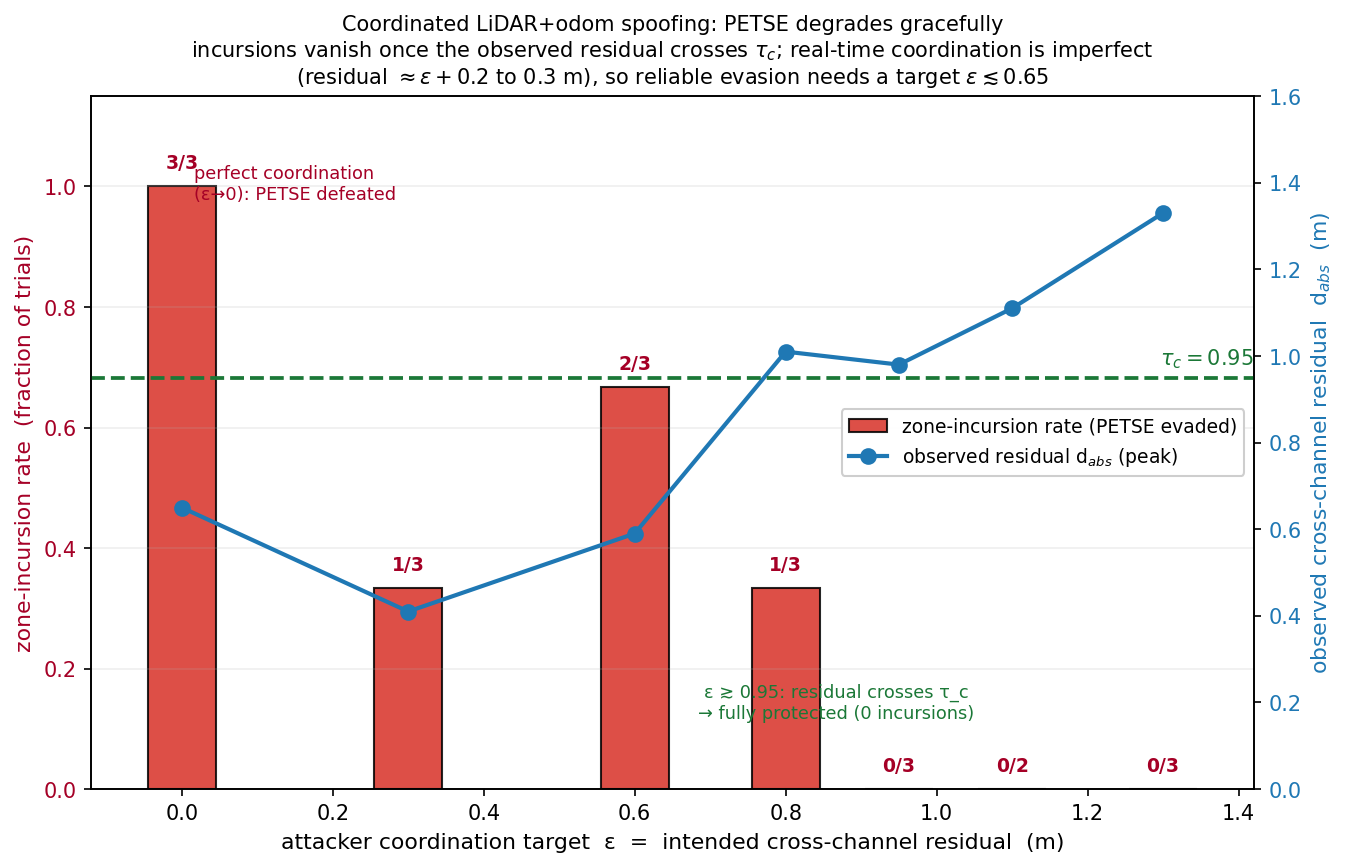
\includegraphics[width=0.95\linewidth]{coord_epsilon_curve.png}
    \vspace{-1.5ex}
    \caption{Coordinated dual-channel (LiDAR\,+\,odometry) spoofing: PETSE degrades
    gracefully. Zone incursions (red, PETSE evaded) fall from 3/3 at perfect coordination
    ($\varepsilon{=}0$) to zero once the observed cross-channel residual $d_{\mathrm{abs}}$
    (blue) crosses the consistency threshold $\tau_c{=}0.95$\,m, which occurs near
    $\varepsilon{\approx}0.8$. Because real-time coordination is imperfect
    ($d_{\mathrm{abs}}\approx\varepsilon+0.2$--$0.3$\,m), reliable evasion requires a target
    $\varepsilon\lesssim0.65$\,m.}
    \label{fig:coord}
\end{figure}

%=====================================================================
\section{Limitations and Discussion}
%=====================================================================

Four limitations are identified.

\textbf{Baseline gap.} No existing method targets the same layer \emph{and} threat model, so our baselines come from adjacent categories (planning, control, monitoring). The comparison reveals how each category fails under execution-time attacks but does not pit PETSE against a peer execution-layer defense---one that, to our knowledge, does not yet exist.

\textbf{Limited evaluation scope.} Simulation used a single Gazebo warehouse with open geometry; narrow corridors, dense clutter, or many closely spaced zones may increase both margin conservatism and false positives. Real-robot trials tested S2--S4 at controlled magnitudes ($1.5\times$ velocity, 0.5\,m offset) but omitted S1 because the LLM refused to produce goals explicitly inside the zone. Platform diversity (differential-drive simulation vs.\ Ackermann hardware) adds some breadth, yet systematic testing across varied maps and stronger attacks remains future work.

\textbf{Bounded-deviation assumption.} Theorem~1 requires the conditions of Lemma~\ref{lem:bounds} to hold. If true velocity exceeds $v_{\max}$, latency exceeds $\tau$, or a spoofing offset is injected faster than the covariance update rate, the margin may be insufficient. PETSE monitors these preconditions and triggers a fail-stop on violation, but fail-stop aborts the mission entirely; a softer degradation path such as online re-routing is not yet implemented.

\textbf{Trusted enforcement layer.} We assume the PETSE node itself is uncompromised. Industrial deployments typically enforce this via hardware isolation (e.g., a dedicated safety PLC or a compute module with read-only firmware). Our prototype runs as a standard ROS node; hardening it to that level is an engineering step we have not yet completed.

%=====================================================================
\section{Conclusion}
%=====================================================================
This article has presented PETSE, an execution-layer safety module that enforces spatial constraints through a dynamic margin summing localization-covariance, tracking-error, latency-drift, and braking-distance bounds. The module operates independently of the LLM and planning stack, preventing forbidden-zone entry even when upstream commands are compromised.

Experimental validation across 1{,}920 Gazebo simulation trials and 140 real-robot runs confirmed zero zone violations under four distinct cyber-physical attack scenarios, with per-cycle overhead below 150\,$\mu$s. The measured safety gap on a physically different platform matched the margin predicted by the proposed formula, confirming cross-platform generality.

The central insight is that safety enforcement belongs at the execution layer, where physical state is directly observable, rather than at the planning layer, where it can only be predicted. PETSE complements planning-level defenses and can be integrated into an existing ROS navigation stack without modifying any upstream component.

Future work will focus on evaluation across diverse facility layouts with narrow corridors, multi-robot coordination scenarios, and alignment with functional safety standards such as IEC~61508.

\bibliographystyle{IEEEtran}
\bibliography{sn-bibliography}

\end{document}
